\section{The mixing law}
\label{app:law}
This appendix proves the mixing law of Sec.~\ref{sec:mixing}: in a reservoir that forgets slowly, a stored function
involves on average as many inputs as the mixing fraction of one input times the memory time. The last part extends
the law to physical channels without a reset, which Appendix~\ref{app:spins} needs.

\subsection{Setting and statement}
We describe the reservoir by the $n$ traceless coordinates $r$ of its state in an orthonormal basis of operators, the
Bloch vector for a qubit. A unitary acts on $r$ as a rotation. In each step the reservoir is reset to a fixed state
with a small probability $p$ and is otherwise rotated by $O(u)$:
\begin{equation}
  r_t=(1-p)\,O(u_t)\,r_{t-1}+p\,b .
  \label{eq:reset}
\end{equation}
Here $b$ represents the reset state, and the inputs $u_t$ are independent and identically distributed. A stored
signal loses a fraction $2p$ of its variance per step, so it lasts about $t_{\mathrm{mem}}=1/(2p)$ steps. Three
conditions make the law hold:
\begin{enumerate}[label=(\arabic*),leftmargin=*,itemsep=2pt,topsep=4pt]
\item \emph{The average step forgets.} The average rotation $A=\mathbb EO$ shrinks every vector: its spectral radius
  is below one.
\item \emph{The inputs scramble.} The only covariance matrices that the random rotations leave unchanged on average,
  $\mathbb E[OXO^{\mathsf T}]=X$, are multiples of the identity.
\item \emph{The input writes.} One input changes the state: $\mathbb E\|(O-A)\mu\|^2>0$ with $\mu=(1-A)^{-1}b$.
\end{enumerate}
The first condition means that only products of inputs can be stored for long, the second that a stored signal
spreads evenly over all directions, and the third that there is something to store. The mixing fraction
\begin{equation}
  s=1-\frac{\|A\|_F^2}{n}
  \label{eq:mixing}
\end{equation}
says how strongly one input turns the stored state. For a unit vector $x$ of random orientation,
$\mathbb E\|(O-A)x\|^2=s$: one input turns a fraction $s$ of a stored signal away from the average rotation. The
fraction lies between 0 and 1, and the first condition makes it positive. If the inputs $u=\pm1$ rotate by
$O=e^{u\theta G}$ with a fixed generator $G$, whose eigenvalues are $i\lambda_1,\dots,i\lambda_n$, the average
rotation is $\cosh\theta G$ and $s=\frac1n\sum_j\sin^2\theta\lambda_j$, which grows as $\theta^2$ for small
turns.

\begin{keybox}
\textbf{Mixing law, precise form.} Assume conditions (1)--(3) and take any fixed linear readout. Pick a stored function
with probability equal to its share of the readout's capacity, and let $D$ be its order. As $p\to0$, the ratio
$D/t_{\mathrm{mem}}$ becomes exponentially distributed with mean $s$, and
\[\mathbb ED=s\,t_{\mathrm{mem}}+O(1).\]
Equivalently, products of more than $x\,t_{\mathrm{mem}}$ inputs carry the share $e^{-x/s}$ of the capacity.
\end{keybox}

\subsection{The idea: a race}
A stored signal is spread evenly over all directions. In each step the current input turns a fraction $s$ of it away
from the average rotation, which adds one input to that part, and the reset removes a fraction $1/t_{\mathrm{mem}}$.
On average $1/s$ steps pass before the next input joins a product, and meanwhile it loses a fraction
$1/(s\,t_{\mathrm{mem}})$ of its weight, so products of more than $K$ inputs carry about
\begin{equation*}
  \Bigl(1-\frac{1}{s\,t_{\mathrm{mem}}}\Bigr)^{K}\approx e^{-K/(s\,t_{\mathrm{mem}})} ,
\end{equation*}
an exponential law with mean $s\,t_{\mathrm{mem}}$. The proof makes this bookkeeping exact.

\subsection{Proof}
\label{app:proof}
The proof works with covariance matrices. Appendix~\ref{sec:order} splits the stationary covariance $\Sigma$ of the state into the
parts $G_k$ carried by products of $k$ inputs and gives their recursion, Eq.~\eqref{eq:recursion}: the mean step
$\mathcal B$ carries a stored product along, and the fluctuating part $\mathcal K$ of the step adds one input to it.
In the reset model the mean step is $\mathcal BX=(1-p)^2AXA^{\mathsf T}$, the full step
$\mathcal TX=(1-p)^2\,\mathbb E[OXO^{\mathsf T}]$, and $\mathcal K=\mathcal T-\mathcal B$. We write $\mathcal B_0$,
$\mathcal T_0$ and $\mathcal K_0$ for the same maps at $p=0$.

\paragraph{Step 1: the stored signal is small and spread evenly.}
The stationary mean is $m=p\,[1-(1-p)A]^{-1}b=p\mu+O(p^2)$, so one input writes the change $(1-p)(O-A)m$, of size
$p$. Its covariance $V$ has the trace $p^2v+O(p^3)$ with $v=\mathbb E\|(O-A)\mu\|^2$, which is positive by
condition (3). The random rotations preserve the trace of a covariance and, by condition (2), leave only the identity unchanged. Since they cannot enlarge a covariance, the identity is a simple fixed point with the projector
$X\mapsto(\Tr X/n)\,1$. On every other direction $(1-\mathcal T)^{-1}$ stays bounded as $p\to0$, while on the identity
it equals $1/[1-(1-p)^2]\approx1/(2p)$. The written covariance therefore piles up along the identity:
\begin{equation}
  \Sigma=(1-\mathcal T)^{-1}V=\frac{pv}{2n}\,1+O(p^2).
  \label{eq:slowcov}
\end{equation}

\paragraph{Step 2: few inputs carry almost nothing.}
The mean step forgets by condition (1), so $(1-\mathcal B)^{-1}$ stays bounded as $p\to0$. The recursion then makes
$G_1=(1-\mathcal B)^{-1}V$ of order $p^2$, and the same holds for every $G_k$ with fixed $k$. Measured against
$\Sigma$, which is of order $p$ and has full rank, any fixed set of orders carries a share of order $p$ of the
capacity of any readout, although the shares of all orders add up to its rank. A long memory consists of products of many
inputs.

\paragraph{Step 3: counting the inputs.}
Call $\mathcal F=(1-\mathcal B)^{-1}\mathcal K$ the order transfer, so that $G_{k+1}=\mathcal FG_k$. At $p=0$ it
leaves the identity unchanged, because $\mathcal K_01=1-AA^{\mathsf T}=(1-\mathcal B_0)1$. Its matching left
eigenvector is the weight
\begin{equation}
  \ell(X)=\Tr[(1-A^{\mathsf T}A)X],\qquad \ell(1)=ns ,
  \label{eq:weight}
\end{equation}
since $\ell(\mathcal F_0X)=\Tr\mathcal K_0X=\ell(X)$ when the rotations preserve the trace. For small $p$ the
eigenvalue one moves to
\begin{equation}
  1-\frac{2}{s}\,p+O(p^2):
  \label{eq:ordereig}
\end{equation}
each step up in order costs a fraction $2p/s=1/(s\,t_{\mathrm{mem}})$ of the weight, as in the race. To see this,
differentiate $(1-\mathcal B)\mathcal F=\mathcal K$ at $p=0$ and apply it to the identity, which gives
$(1-\mathcal B_0)\mathcal F_0'1=-2\cdot1$. Its trace is the weight $\ell(\mathcal F_0'1)=-2n$, and dividing by
$\ell(1)=ns$ gives the rate $2/s$.

To turn the eigenvalue into a distribution, weigh order $k$ with $e^{-\lambda pk}$. Summing the recursion gives
$\sum_kz^kG_k=z(1-z\mathcal F)^{-1}G_1$, and as $z=e^{-\lambda p}$ approaches one, only the eigenvalue of
Eq.~\eqref{eq:ordereig} makes the inverse large. With $\ell(G_1)=p^2v+O(p^3)$ and $\beta=2/s$,
\begin{equation}
  \sum_{k\ge1}e^{-\lambda pk}G_k=\frac{pv}{2n}\,\frac{\beta}{\lambda+\beta}\,1+O(p^2).
  \label{eq:laplace}
\end{equation}
Divided by Eq.~\eqref{eq:slowcov}, this is $\beta/(\lambda+\beta)$, the Laplace transform of an exponential
distribution of $pD$ with rate $\beta$. So $D/t_{\mathrm{mem}}=2pD$ is exponential with mean $s$. Because both
covariances are multiples of the identity to leading order, the same holds for the share of the capacity of any
readout. Finally, $\sum_kkG_k=(1-\mathcal F)^{-1}\Sigma=\Sigma/(\beta p)+O(p)$ gives
$\mathbb ED=s\,t_{\mathrm{mem}}+O(1)$.

\paragraph{Two technical points.}
The eigenvalue one of $\mathcal F_0$ is simple: a fixed point of $\mathcal F_0$ satisfies $\mathcal T_0X=X$ and is
therefore a multiple of the identity, and $\ell(1)>0$ rules out a Jordan chain. For $p>0$ every eigenvalue of
$\mathcal F$ lies inside the unit circle, by a Perron--Frobenius argument: $\mathcal F$ maps positive matrices to
positive matrices, and so does $(1-\mathcal F)^{-1}=1+(1-\mathcal T)^{-1}\mathcal K$. The eigenvalues of
$\mathcal F_0$ therefore lie in the closed unit disk, only the simple one equals one, and only the eigenvalue of
Eq.~\eqref{eq:ordereig} makes the sum diverge.

\subsection{When the law needs one slow direction}
Condition (2) matters. Let a classical flag, set by the reset state and never changed, select one of two qubit
rotations about $Z$, by $\pm\pi/6$ or by $\pm\pi/3$, and let the reset state put the flag in either value with
probability $\tfrac12$ and the qubit along $+X$ in both. Each sector obeys the law with its own mixing fraction,
$1/4$ and $3/4$, and a single $Y$ readout sees their mixture, weighted by the variance each sector stores. The
gentler sector stores more, so as $p\to0$ products of more than $x\,t_{\mathrm{mem}}$ inputs carry the share
$w\,e^{-4x}+(1-w)\,e^{-4x/3}$ with $w=0.82$, which exact moments reproduce. One observable then shows two order
scales.

\subsection{Physical channels without a reset}
\label{app:physical}
A physical channel does not reset to a prescribed state, but the proof used the reset only through three facts: one
covariance direction is slow, it leaks at a small rate, and the mean step forgets everything else. The same three
steps therefore prove the law for general channels. Appendix~\ref{app:spins} uses this version, and readers interested in the reset model can skip it.

\emph{Setting.} One step is $r_t=A_u(\epsilon)r_{t-1}+b_u(\epsilon)$ on the coordinates that the inputs can reach,
with a small leak $\epsilon$, and $\mathcal B$, $\mathcal T$ and $\mathcal K$ are formed from $A_u$ as before. We
assume:
\begin{enumerate}[label=(\roman*),leftmargin=*,itemsep=2pt,topsep=4pt]
\item $A_u$ and $b_u$ depend smoothly on $\epsilon$ in mean square, and $b_u$ vanishes at $\epsilon=0$.
\item The mean step forgets at $\epsilon=0$: $\mathbb EA_u(0)$ has spectral radius below one.
\item The channel is mean-square stable for small $\epsilon>0$.
\item One covariance direction is slow: $\mathcal T$ has a simple eigenvalue $1-\kappa\epsilon+O(\epsilon^2)$ with
  $\kappa>0$ and no other eigenvalue near one. At $\epsilon=0$ its right eigenvector is a positive matrix $Q$, and its
  left eigenvector is a weight $\ell$ that is nonnegative on positive matrices, with $\ell(Q)=1$.
\item The input writes along it: the change written by one input, of order $\epsilon$, has covariance
  $\epsilon^2V_*+O(\epsilon^3)$ with $\ell(V_*)>0$.
\end{enumerate}
The reset model is the case $\epsilon=p$, $\kappa=2$, $Q=1$ and $\ell=\Tr/n$. Condition (iv) concerns the
covariance that the random steps carry, not the number of slow modes: at a fixed amplitude the inputs turn the 99
slow dark modes of a shared channel with opposite phases differently in each step and spread a stored signal over
all of them, so that one covariance direction stays slow. With several slow directions, each mixes at its own rate,
as in the example above. Conditions (ii) and (iii) say that the reservoir forgets its starting state on average and in
mean square, (iv) that the random steps spread a stored signal over the slow modes faster than it leaks, and (v) that
the surviving direction is written.

\begin{keybox}
\textbf{Mixing law without a reset.} Under (i)--(v) the mixing fraction $s=\ell(\mathcal K_0Q)$ is positive and at
most one, and $\epsilon D$ becomes exponentially distributed with rate $\kappa/s$. The mean order is
$s/(\kappa\epsilon)+O(1)$: the mixing fraction times the memory time $1/(\kappa\epsilon)$.
\end{keybox}

\emph{Proof.} Steps 1 and 2 carry over. The stationary mean is of order $\epsilon$ by (i) and (ii), and the slow
eigenvalue piles the written covariance up along $Q$,
\begin{equation*}
  \Sigma=\epsilon\,\frac{\ell(V_*)}{\kappa}\,Q+O(\epsilon^2),
\end{equation*}
and every fixed order carries a covariance of order $\epsilon^2$. For the memory of a readout with several features we
also need $Q$ to have full rank on what the readout measures, which holds trivially for one observable. In step 3,
$\mathcal F_0$ has the same fixed points as $\mathcal T_0$, so $Q$ spans them, and $\ell\circ(1-\mathcal B_0)$ is its
left eigenvector, with value $\ell(\mathcal K_0Q)=s$ on $Q$. Differentiating $(1-\mathcal B)\mathcal F=\mathcal K$ at
$\epsilon=0$ and applying it to $Q$ gives $(1-\mathcal B_0)\mathcal F_0'Q=\mathcal T_0'Q$, whose weight
$\ell(\mathcal T_0'Q)=-\kappa$ is the rate of the slow eigenvalue of $\mathcal T$. The order eigenvalue is
therefore $1-(\kappa/s)\epsilon+O(\epsilon^2)$, and the Laplace transform follows as before. It remains to show that $s$ is positive, which also makes the eigenvalue
simple. Because $\mathcal K_0$ maps positive matrices to positive matrices and $\ell$ is nonnegative on them,
$\ell(\mathcal B_0Y)\le\ell(\mathcal T_0Y)=\ell(Y)$ for every positive $Y$, so $0\le\ell(\mathcal
B_0^j\mathcal K_0Q)\le s\le1$ for every $j$. If $s$ vanished, the series $\mathcal F_0=\sum_j\mathcal B_0^j\mathcal
K_0$ would give $\ell(\mathcal F_0Q)=0$, which contradicts $\mathcal F_0Q=Q$ and $\ell(Q)=1$.

\emph{The spin reservoirs.} For three spins the certificates of Appendix~\ref{app:spins} check these conditions. For
five spins we check the law instead of the conditions: Eq.~\eqref{eq:recursion} gives the order distribution exactly,
and it follows the law (below).

\subsection{Numerical check}
Figure~\ref{fig:law} compares the law with exact moments. Beyond the reservoir shown, we tested 24 reservoirs and
readouts in dimensions two to four: two families of three random unitaries, two reset states (a basis state and a
random pure state) and two readouts (all coordinates or one random direction). The largest deviation from the law shrinks in proportion to $p$, from 0.08 at $p=3\%$ to 0.003 at
$p=0.1\%$. The five-spin reservoir follows the law as well (Fig.~\ref{fig:mixing}c): at the largest memories
computed, $s\,t_{\mathrm{mem}}\approx20$, products of more than $K$ inputs carry the share
$e^{-K/(s\,t_{\mathrm{mem}})}$ of the capacity to within 0.14.

\begin{figure}[t]
\centering
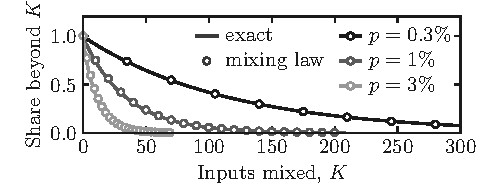
\includegraphics[width=\columnwidth]{figures/figA_law.pdf}
\caption{\textbf{The mixing law.} Share of the capacity carried by products of more than $K$ inputs, for one qubit
that is reset with a small probability $p$ in each step. Lines: exact, circles: the exponential law of
Theorem~\ref{thm:law}.}
\label{fig:law}
\end{figure}

\section{One qubit in closed form}
\label{app:qubit}
This appendix solves the qubit of Sec.~\ref{sec:writing} exactly. At a fixed turn per input the number of inputs
mixed grows as the memory time. A turn that shrinks as the square root of the relaxation rate keeps it finite, and
the stored signal is largest at an intermediate turn.

\paragraph{The model.}
The qubit relaxes towards $+X$ at a rate $\epsilon$, through the jump $\sqrt\epsilon\,|{+x}\rangle\langle{-x}|$, and
the input $u=\pm1$ turns it about $Z$ by $u\theta$ per unit time. Each input lasts one unit of time, and the qubit is
read along $Y$. In the Bloch plane,
\begin{equation}
  \dot x=-\epsilon(x-1)-u\theta y,\qquad \dot y=u\theta x-\tfrac12\epsilon y .
  \label{eq:bloch}
\end{equation}
Over one step this is a linear map of $(x,y)$ plus an offset. For $u=+1$ the map has the form
$\bigl(\begin{smallmatrix}a&-b\\ b&d\end{smallmatrix}\bigr)$ and the offset is $(f,g)$. For $u=-1$ the signs of $b$
and $g$ flip. The input-averaged step is therefore diagonal, the stationary mean lies on the $X$ axis at
$m=f/(1-a)$, and each input writes $u\,v$, with $v=bm+g$, along the measured axis $Y$.

\paragraph{How the orders arise.}
The averaged step keeps the two axes apart, while the input-dependent part swaps them. A signal written into $Y$ must
pass through $X$ and back to pick up more inputs, so $Y$ carries only odd orders. By the
recursion~\eqref{eq:recursion}, covariance passes from $Y$ to $X$ with the factor $b^2/(1-a^2)$ and back with
$b^2/(1-d^2)$. Call the product of the two factors $\chi$. Order $2j+1$ then carries the share $(1-\chi)\chi^j$ of
the capacity of $Y$, and
\begin{equation}
  \mathbb ED=\frac{1+\chi}{1-\chi},\qquad \mathrm{Var}\,Y=\frac{v^2}{(1-d^2)(1-\chi)} .
  \label{eq:qubit}
\end{equation}
Single past inputs carry the share $d^2(1-\chi)$.

\paragraph{Fixed turn.}
Let the relaxation slow down, $\epsilon\to0$, at a fixed angle $\theta$ with $\sin\theta\neq0$. Then
$1-\chi=3\epsilon/\sin^2\theta+O(\epsilon^2)$: the order grows as $1/\epsilon$, $\epsilon D$ becomes exponentially
distributed with rate $3/(2\sin^2\theta)$, and the share of single inputs vanishes, even for exact expectation values.

\paragraph{Gentle writing.}
If instead $\theta^2/\epsilon$ approaches a constant $\nu$, then to first order $a=1-(1+\nu/2)\epsilon$ and
$d=1-(1+\nu)\epsilon/2$, with $b\approx\theta$ and $f\approx\epsilon$, and as $\epsilon\to0$
\begin{equation}
  \begin{aligned}
    \chi&\to\frac{\nu^2}{(\nu+2)(\nu+1)},\\
    \mathrm{Var}\,Y&\to\frac{4\nu}{(\nu+2)(3\nu+2)} .
  \end{aligned}
  \label{eq:qubitlimit}
\end{equation}
The mean order stays finite, and single past inputs keep the share $1-\chi$. Their recall beyond delay $\tau$ is the
fraction $d^{2\tau}$ of the total, so the range that holds 90\% of it grows as $1/\epsilon$:
$\epsilon\tau_{90}\to\ln10/(1+\nu)$.

\paragraph{The best turn.}
The signal of Eq.~\eqref{eq:qubitlimit} is largest at $\nu=2/\sqrt3$ (Fig.~\ref{fig:mixing}d). For $\nu\gg1$ it
vanishes as $4/(3\nu)$, because later inputs scramble earlier ones. For $\nu\ll1$ it vanishes as $\nu$, because each input writes too
little. Among power laws $\theta\propto\epsilon^\alpha$, only $\alpha=1/2$ keeps a finite signal: the turn must fall as
the square root of the relaxation rate, that is, as one over the square root of the memory time. Direct propagation
of the density matrix reproduces all these expressions.

\section{Three spins at strong loss}
\label{app:spins}
\begin{keybox}
\textbf{What we prove.} Take three spins with one shared channel of opposite phases, Eq.~\eqref{eq:H3}, the four
Hamiltonians H1--H4 of Table~\ref{tab:spins}, and every Hamiltonian whose three couplings lie in a small box around
theirs. As $\gamma$ grows:
\begin{itemize}[leftmargin=*,itemsep=2pt,topsep=4pt]
\item At a fixed input amplitude, the order of the memory of $X_1$, divided by $\gamma$, becomes exponentially
  distributed, and the signal in $X_1$ falls as $1/\gamma$ (boxes of half-width 1/32).
\item With the amplitude scaled as $8/\sqrt\gamma$, single past inputs keep a finite share of the capacity of $X_1$,
  and the range of delays that holds 90\% of their recall grows in proportion to $\gamma$ (boxes of half-width 1/512).
\end{itemize}
\end{keybox}

\paragraph{Idea.}
At strong loss, one step of the full master equation is a rotation of the three dark states, up to corrections of
order $\epsilon=1/\gamma$. At a fixed amplitude the two signs of the input rotate the dark states differently. The
stored covariance then has a single slow direction, and the mixing law without a reset applies
(Appendix~\ref{app:physical}). With gentle writing both signs give almost the same rotation. The signal is
written on the scale of the leak and collects in six slow directions, which we follow explicitly. Both arguments end
in finitely many strict inequalities, which a computer checks with rigorous error bounds.

\paragraph{Model and computations.}
The three spins evolve under
\begin{equation}
  H_\eta(u)=\sum_{i<j}J_{ij}X_iX_j+\tfrac12\sum_iZ_i+\tfrac{3+\eta u}{4}\sum_iX_i
  \label{eq:H3}
\end{equation}
with one jump $\sqrt\gamma\,(\sigma_1^--\sigma_2^--\sigma_3^-)$, steps of $\Delta t=1/2$ and signs $u=\pm1$, at
$\eta=1$ (fixed amplitude) or $\eta=8/\sqrt\gamma$ (gentle writing): the field of gentle writing
(Appendix~\ref{sec:methods-slow}) with signs in place of uniform inputs, with the same mean and the same largest change
$\eta/4$. The couplings of the four Hamiltonians H1--H4
are drawn from fixed seeds. For each loss rate we exponentiate the full generator for both signs, solve the
stationary moment equations and evaluate Eq.~\eqref{eq:recursion} for $X_1$ until 99.99\% of its memory is accounted
for. The range $\tau_{90}$ is the smallest delay beyond which less than a tenth of the recall of single inputs
remains.

\paragraph{Both regimes.}
Figure~\ref{fig:spins} shows the two regimes of the box for H3. Gentler writing trades signal for readability, as for
the qubit: at $\eta_0=8$ single inputs keep between
8\% and 81\% of the capacity of $X_1$ for the four Hamiltonians (Table~\ref{tab:spins}), and for H3 this share rises to
67\% at $\eta_0=2$, with a signal 25 times smaller.

\begin{figure}[t]
\centering
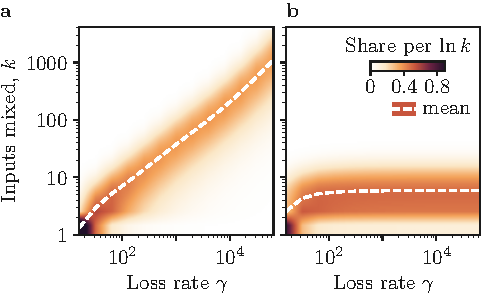
\includegraphics[width=\columnwidth]{figures/figC_spins.pdf}
\caption{\textbf{Three spins, both regimes.} Share of the capacity of $X_1$ carried by products of $k$ inputs
(colour) against the loss rate, for one shared channel with opposite phases (Hamiltonian H3). Dashed: the mean. At a
fixed input strength the number of inputs mixed grows with the loss (a), while with gentle writing it stays small (b).}
\label{fig:spins}
\end{figure}

\begin{table}[t]
\caption{\label{tab:spins}Strong-loss limits for $X_1$ in the four three-spin reservoirs. Fixed amplitude: rate of
the exponential law of the order divided by $\gamma$ (certified). Gentle writing: share of single past inputs and
range of their recall divided by $\gamma$, evaluated at $\gamma=2^{16}$.}
\centering\footnotesize
\begin{tabular}{lccc}
\toprule
 & rate & single-input share & range$/\gamma$\\\midrule
H1 & 78.6 & 0.81 & 0.50\\
H2 & 91.7 & 0.29 & 0.18\\
H3 & 61.4 & 0.08 & 0.24\\
H4 & 132.5 & 0.14 & 0.50\\
\bottomrule
\end{tabular}
\end{table}

\paragraph{One step at strong loss.}
The jump $\sqrt\gamma\,(\sigma_1^--\sigma_2^--\sigma_3^-)$ leaves three dark states: the state with no excitation
and the two single-excitation states with amplitudes $(0,1,-1)/\sqrt2$ and $(2,1,1)/\sqrt6$, which are orthogonal to
the phases of the channel. It empties every other state, so at unit loss rate only the nine operators on the dark
states do not decay. Let $R$ embed these nine coordinates into the full operator space and $R^\flat$ project back
along the decaying operators. Expanding one step in $\epsilon$ gives
\begin{equation}
  E_u=R\,e^{\Delta t\,R^\flat\mathcal H_uR}R^\flat+\epsilon Z_u+O(\epsilon^2),
  \label{eq:slowstep}
\end{equation}
where $\mathcal H_u$ is the commutator with the Hamiltonian of input $u$. The first term rotates the dark states. The
correction $Z_u$ collects the brief excursions into bright states: one at the start of the step, one at its end, and
the leak of Eq.~\eqref{eq:reduced} in between.

\paragraph{Fixed amplitude.}
At $\eta=1$ the dark rotations $O_u$ of the two signs differ, and the computer checks the conditions of the mixing law
without a reset on the eight traceless dark coordinates. The average rotation forgets. The identity is the only covariance that the random rotations leave unchanged. Three constants from the first-order terms of
Eq.~\eqref{eq:slowstep} are positive: the strength with which an input writes, the rate $\kappa$ at which the slow
covariance leaks, and the mixing fraction $s_0=1-\|\mathbb EO_u\|_F^2/8$. The law then gives an exponential
distribution of the order divided by $\gamma$, with rate $\kappa/s_0$ (Table~\ref{tab:spins}), and the variance of
$X_1$ falls as $\epsilon$. A change $r$ of the couplings moves each dark rotation by at most $3r$, which lets the
checks cover the boxes of half-width 1/32.

\paragraph{Gentle writing.}
At $\eta=8\sqrt\epsilon$ both signs give the same leading rotation $E$, generated by the static part of the dark
Hamiltonian. The input enters at order $\sqrt\epsilon$ and the leak at order $\epsilon$. Expanding the step to this order
gives the mean step $E+\epsilon E_1$ and the input-dependent part $u\sqrt\epsilon\,\Delta_1$.

\emph{Where the signal goes.} The rotation $E$ turns each of the three planes of coherence between the dark energy
levels by its own angle, set by an energy gap, and the six phases of these turns differ from each other and from one.
So $E$ leaves only the populations unchanged, and on them $E_1$ generates a slow population dynamics with a unique stationary state
$m_*$. An input therefore writes $\pm\sqrt\epsilon\,v$ with $v=\Delta_1m_*$, which lies in the coherence planes: a new
input first turns a population into a coherence.

\emph{Six slow directions.} The covariances that $E$ leaves unchanged form a six-dimensional space: the three
covariances of the two population coordinates and one isotropic covariance in each coherence plane. Over $1/\epsilon$
steps a covariance in this space changes under two generators, both certified stable. $K_B$ describes how the mean
step lets a stored signal decay, and $K_T$ adds the random signs of later inputs, which turn a stored signal into
products. With $P_6$ the projection onto the six directions, the single-input part of the stored covariance and the
full covariance approach $W_*=-K_B^{-1}P_6(vv^{\mathsf T})$ and $\Sigma_*=-K_T^{-1}P_6(vv^{\mathsf T})$.

\emph{Limits.} With $a$ the coordinates of $X_1$, the share of single past inputs in the memory of $X_1$ tends to
$a^{\mathsf T}W_*a/a^{\mathsf T}\Sigma_*a$. After $t/\epsilon$ steps the remaining single-input recall is the fraction
$a^{\mathsf T}e^{tK_B}W_*a/a^{\mathsf T}W_*a$, which crosses 0.1 once, and the crossing is the range divided by $\gamma$.
The certificates show $a^{\mathsf T}W_*a>0$, and since $\Sigma_*\succeq W_*$ the share is positive. In the boxes of
half-width 1/512 the six angles stay separated and both generators stay stable, so the limits stay positive.

\paragraph{Why coherence carries the memory.}
Returning bright population to the dark subspace after every step leaves the leading terms of the scaled step
unchanged, so it keeps the same limits. Dephasing in the dark energy basis, by contrast, removes the coherence planes
into which $v$ writes. Restricted to populations, the two signs then differ only at order $\epsilon^{3/2}$, because the
response of a population at order $\sqrt\epsilon$ is a coherence, while the populations still follow the slow
population dynamics. A new input thus writes a vector of size $\epsilon^{3/2}$, the slow dynamics sum its square over
$1/\epsilon$ steps, and the stored signal is of order $\epsilon^2$: the collapse as $1/\gamma^2$ of
Sec.~\ref{sec:writing}. Numerically, applying the loss-only projector $\mathcal P$ after every step, with or without
dephasing in the energy basis of the projected Hamiltonian, the variance of $X_1$ stays between $10^{-4}$ and
$2\times10^{-3}$ from $\gamma=2^8$ to $2^{18}$ when the coherences are kept and falls as $\gamma^{-2}$, by six orders
of magnitude, when they are erased. At a fixed input amplitude it falls as $1/\gamma$.

\paragraph{What the computer checks.}
The attached archive \texttt{spin\_certificates.zip} contains the generators, the exact couplings and the interval
programs. They enclose every quantity above in intervals with rigorous rounding (ball arithmetic of Arb, python-flint
0.9.0) and check each strict inequality of this appendix at 256 bits, and at 192 bits they reproduce the archived
enclosures. A second program, sharing no routine with
them, builds the full finite-rate maps and extrapolates to infinite loss. It agrees with
the certified rates and limiting recalls to better than one part in a million.

\section{Numerical details and supporting checks}
\label{app:numerics}
This appendix backs the main text: each paragraph names the section it supports, says what we checked and gives what
is needed to reproduce it.

\paragraph{Recall and memory (Sec.~\ref{sec:clock}).}
Figures smooth recall curves for display only: each delay is averaged with its neighbours, with weights that fall
linearly to zero at a fifth of the delay, and no sum uses the smoothed values. The maps of Fig.~\ref{fig:clock}a,b are
computed at $\gamma=0.1$, 0.25 and $2^{-1}$ to $2^6$ in powers of two and interpolated by shifting each recall profile
along the delay. Figure~\ref{fig:clock}c stops one and two shared channels at $\gamma=64$, where their recall at the
full amplitude starts to reach past the 300 delays we sum. Summed over all delays with exact moments
(Appendix~\ref{sec:order}), their memory keeps rising up to $\gamma=256$. With gentle writing, delays beyond 300 add
about 1\% to the memory of opposite phases.

\paragraph{Dark states (Sec.~\ref{sec:clock}).}
Both tests act on the 100 dark coordinates. For the dark-state model we write $\mathcal P=RR^\flat$ with $R^\flat R=1$,
where $R$ embeds the dark coordinates $\alpha$, evolve $\alpha$ under Eq.~\eqref{eq:reduced} and record the same 45
features of the full state $(R-\mathcal S\mathcal H(u)R/\gamma)\,\alpha$. The readout is trained on them exactly as for
the full reservoir, and the model has no fitted parameter (Fig.~\ref{fig:darkmodel}a). For the erasure test we replace
the dark coordinates after every step by their time average, $r\mapsto r-RR^\flat(r-\bar r)$. The control erases the
dark subspace rotated by a random product of single-spin unitaries. Recall is measured at delays 1 to 100 with 800
training, 200 validation and 800 test inputs (Fig.~\ref{fig:darkmodel}b).

The leak out of the dark states falls exactly as $1/\gamma$: for one shared channel $\gamma\bar\kappa$ approaches
$\kappa_{\mathrm c}=2.945$ from $\gamma=512$ on, so $t_{\mathrm f}$ grows in proportion to $\gamma$, while it levels off
near 56 steps with opposite phases and near 110 with pairwise loss. The second-order calculation of
Eq.~\eqref{eq:reduced} gives the same $\kappa_{\mathrm c}$ at five spins and 1.4, 2.1 and 3.4 at three, four and six
spins: the size of the reservoir sets only the strength of the leak.

\begin{figure}[t]
\centering
\includegraphics[width=\columnwidth]{figures/figD_dark.pdf}
\caption{\textbf{Dark states hold the memory.} One shared channel.
\textbf{a}~The dark states alone (circles), with no fitted parameter, reproduce the recall of the full reservoir
(lines).
\textbf{b}~Erasing the dark states after every step destroys the memory, while erasing a rotated copy of the same size
leaves most of it (dark line: intact reservoir, $\gamma=16$).}
\label{fig:darkmodel}
\end{figure}

\paragraph{Time to forget and phases (Sec.~\ref{sec:mixing}).}
We compute $t_{\mathrm f}$ at $\eta=1$, $\tfrac12$, $\tfrac14$ and $\tfrac18$, for $\gamma$ from $2^{-8}$ to $2^6$ with
local loss and from $2^{-2}$ to $2^{12}$ with opposite phases. The collapses of Fig.~\ref{fig:mixing}a do not depend on
how the time to forget is defined: with the slowest mode in place of the mean rate they hold to within 11\% wherever
forgetting takes more than four steps, and they hold as well with the input on one spin. Weakening the input moves the
best loss rate: on one reservoir with exact moments, the memory peak of local loss moves from $\gamma\approx1/16$ at
$\eta=1$ to $1/64$ at $\eta=\tfrac18$, and the best memory rises from 16 to 39 units.

The write per input of Fig.~\ref{fig:mixing}b is $2\|R^\flat[E(\tfrac34)-E(\tfrac14)]r_*\|$ at the stationary state
$r_*$ of the equal-phase channel, for the input patterns $(1,\dots,1)$ and $\sqrt2\cos(2\pi i/5)$ multiplying $X_i$.
Along the phases it falls as $1/\gamma$, to 0.003 at $\gamma=128$, while across them it falls only slowly, to 0.18. Opposite
phases are the equal-phase channel with the field on spins 4 and 5 reversed, up to a relabelling of the random
couplings (a turn of these spins by $\pi$ about $Z$).

\paragraph{Orders and capacities (Secs.~\ref{sec:mixing} and~\ref{sec:writing}).}
The order distribution of Eq.~\eqref{eq:recursion} uses six-point Gauss--Legendre quadrature for the expectations over
the input and solves the equations $X-\bar AX\bar A^{\mathsf T}=C$ in the eigenbasis of $\bar A$. The shares of the 45 features are summed until the rest falls below $10^{-8}$, or until successive orders shrink at a settled ratio, whose
geometric tail we add. The linear recall follows from the same moments,
$C_\tau=c_\tau^{\mathsf T}\Sigma_y^{-1}c_\tau/\mathrm{Var}\,u$ with $c_\tau$ the covariance of the features with
$u_{t-\tau}$ and $\Sigma_y$ their covariance, and reproduces the simulated memories to a median of 2\%. Three steps of
inverse iteration on $\mathcal T$, from the input's covariance $V$ and from the identity, give $t_{\mathrm{mem}}$, $Q$
and $\ell$. Loss rates run in powers of four over the ranges of Fig.~\ref{fig:mixing}c, and with gentle writing to
16384 and $1/4096$, on four reservoirs, two at the largest memory times. With local loss the mean order follows the law
as well, within 2.2 of $s\,t_{\mathrm{mem}}$ up to $s\,t_{\mathrm{mem}}=18$.

\paragraph{Measurement (Sec.~\ref{sec:price}).}
We measure the signal by the variance of a feature over the test inputs, averaged over the features. Gentle writing
makes it fainter: with opposite phases it falls from $8\times10^{-5}$ at the full amplitude to $5\times10^{-6}$, against
$7\times10^{-5}$ with local loss and gentle writing at $\gamma=1/32$. Restarting each run from $|00000\rangle$, as the
replay does, raises these to $4\times10^{-5}$ and $1.2\times10^{-4}$. At the full amplitude the signal of the
equal-phase channel falls from $2\times10^{-4}$ at $\gamma=1$ to $4\times10^{-7}$ at $\gamma=64$, which is why this
channel loses memory as the loss grows once measurements are counted.

The replayed range $\tau_{90}$ grows with the clock, though more slowly: along the gentle line of opposite phases from
about 30 steps at $\gamma=16$ to 130 at $\gamma=256$. The budget sets the best loss rate: at $10^{10}$ preparations
times replayed steps the optimum of the equal-phase channel moves from $\gamma=1$ to about 16, with 17 units, while
opposite phases with gentle writing peak near $\gamma=64$ with 25. Below the crossings the full amplitude wins: at
$10^4$ preparations it keeps 11 units with local loss and 8 with opposite phases, against 9 and 3 with gentle writing.
With the input on one spin, which writes more gently by itself, the crossings move to about $3\times10^5$ and
$4\times10^6$ preparations. With the full history, eight times more training inputs change the sampled memory by less
than 1.3 units.

For the matched clock of Fig.~\ref{fig:sampling}b we find, for every shape and reservoir, the loss rate at which
$t_{\mathrm{leak}}=32$ steps, at weak loss without protected operators and at strong loss with them, and run the
reservoir there with $\eta=\sqrt{4/32}$. The write is $-i[H_{\mathrm{in}},\rho_*]$ with $H_{\mathrm{in}}=h\sum_iX_i$ and
$\rho_*$ the stationary state, projected spectrally onto the slow modes: the protected ones, or without protected
operators those decaying at most four times faster than the slowest. The memory that survives $10^6$ preparations
rises with the write, from 0.3 units for the shared channels to 17 for local loss, and power laws fitted within the
shapes without and with dark states (dotted in Fig.~\ref{fig:sampling}b) have exponents 2.0, as linear accumulation of
the write predicts, and 1.5.

\paragraph{Ordinary noise (Sec.~\ref{sec:conclusion}).}
Adding local loss $\sqrt{\gamma_{\mathrm{loc}}}\,\sigma_i^-$ to a shared channel gives
$\bar\kappa=\kappa_{\mathrm c}/\gamma+\kappa_{\mathrm l}\gamma_{\mathrm{loc}}$, where to first order $\kappa_{\mathrm l}$
is the trace of the added dissipator on the 99 slow dark modes divided by 99, $140/99\approx1.414$. Local dephasing
$\sqrt{\gamma_\phi}\,Z_i$ adds $\kappa_\phi\gamma_\phi$ with $\kappa_\phi=403.2/99\approx4.073$, and the full spectra
reproduce both coefficients to within 0.2\%. A time to forget of at least $T$ steps,
$\kappa_{\mathrm c}/\gamma+\kappa_{\mathrm l}\gamma_{\mathrm{loc}}\le1/(\Delta t\,T)$, then needs
$\gamma/\gamma_{\mathrm{loc}}\ge4\kappa_{\mathrm c}\kappa_{\mathrm l}\,\Delta t^2T^2\approx4.2\,T^2$, or $12\,T^2$ for
dephasing.
